\documentclass{article}

\usepackage{neurips_2026}

\usepackage[utf8]{inputenc}
\usepackage[T1]{fontenc}
\usepackage{hyperref}
\usepackage{url}
\usepackage{booktabs}
\usepackage{amsfonts}
\usepackage{amsmath}
\usepackage{nicefrac}
\usepackage{microtype}
\usepackage{xcolor}
\usepackage{graphicx}
\usepackage{subcaption}
\usepackage{multirow}

\title{Hyperbolic Geometry in Platonic Representations}

\author{%
  Anonymous Author(s) \\
  Affiliation \\
  Address \\
  \texttt{email}
}

\begin{document}
\maketitle

\begin{abstract}
The Platonic Representation Hypothesis posits that foundation models converge toward a shared representation of reality, but does not characterize its geometry. We show that the inter-class distance structure of vision models, causal language models, and text embedding models is \emph{tree-like}---consistent with hyperbolic geometry---and that the training \emph{objective}, not the modality, determines the type of tree learned. Using Gromov $\delta$-hyperbolicity on 22 vision models, 9 causal LMs, and 8 text embedding models evaluated on 1{,}000 ImageNet classes, we find: (1)~self-supervised vision models (DINOv2-L: $\delta = 0.067$) and causal LMs (GPT-2 XL: $\delta = 0.073$) achieve the lowest $\delta$, learning emergent hierarchies that do not align with WordNet; (2)~contrastive models---both vision (CLIP) and text (BGE, GTE, E5)---learn WordNet-aligned hierarchies with higher $\delta$; (3)~controlled experiments confirm $\delta$ reflects learned hierarchy: random weights increase $\delta$ by 65--144\%, non-hierarchical fine-tuning by 19--91\%, and $\delta$ emerges progressively across transformer layers (46--60\% decrease); (4)~$\delta$ is a \emph{practical decision tool}: a parameter-free post-hoc Poincar\'{e} projection of frozen-backbone features improves nearest-centroid classification ($r = -0.629$ with $\delta$, $n = 60$) and few-shot learning ($r = -0.604$, $n = 60$), with gains restricted to settings that have asymmetry between query (sample) and target (prototype). Our findings establish tree-like geometry as a universal property of learned representations whose practical consequences---when to use hyperbolic distances and when not to---are predicted by a zero-cost geometric diagnostic.
\end{abstract}

%% ============================================================
\section{Introduction}
\label{sec:intro}
%% ============================================================

The Platonic Representation Hypothesis (PRH)~\citep{huh2024platonic} provides evidence that foundation models converge toward a shared representation of reality as they scale. The PRH measures \emph{that} models converge, but not \emph{to what geometry}. Yet the structure of reality is fundamentally hierarchical: objects belong to categories, categories to superordinate classes. The natural geometry for hierarchies is hyperbolic~\citep{nickel2017poincare, sarkar2011low}.

We ask: \emph{does the platonic representation have hyperbolic geometry?} We measure Gromov $\delta$-hyperbolicity~\citep{gromov1987hyperbolic} directly on the Euclidean embeddings of 39 models---22 vision, 9 causal LM, 8 text embedding---spanning five training paradigms.

\textbf{Contributions.}
\begin{enumerate}[topsep=0pt,itemsep=0pt]
\item Tree-like geometry is \textbf{universal across modalities}. All 39 models have $\delta$ well below Euclidean and spherical references; the training objective, not the modality, determines the degree and type of tree-likeness.
\item \textbf{Causal evidence} that $\delta$ reflects learned semantic hierarchy: random weights (+65--144\%), non-hierarchical fine-tuning (+19--91\%), and progressive layer-wise emergence (--46 to --60\%) all alter $\delta$ in directions consistent with hierarchy formation.
\item Causal language models, contrary to prior assumption, are also tree-like when evaluated on the same 1{,}000 ImageNet classes (GPT-2 XL: $\delta = 0.073$, comparable to the best vision SSL models).
\item $\delta$ is a \textbf{practical decision tool} for post-hoc hyperbolic projection. On 12 vision backbones $\times$ 5 datasets, the hyperbolic advantage in nearest-centroid classification ($r = -0.629$, $n = 60$) and 5-way 5-shot few-shot ($r = -0.604$, $n = 60$) scales with backbone $\delta$, while settings without query/target asymmetry (sample-to-sample retrieval) show no advantage---a result consistent with the geometric mechanism.
\end{enumerate}

%% ============================================================
\section{Background}
\label{sec:background}
%% ============================================================

\paragraph{Gromov $\delta$-hyperbolicity.} A metric space is $\delta$-hyperbolic~\citep{gromov1987hyperbolic} if for any four points $x, y, z, w$, ordering the three pairwise sums $S_1{=}d(x,y){+}d(z,w)$, $S_2{=}d(x,z){+}d(y,w)$, $S_3{=}d(x,w){+}d(y,z)$ as $S_{\max} \ge S_{\text{mid}} \ge S_{\min}$,
\begin{equation}
\delta = \max_{x,y,z,w} \frac{S_{\max} - S_{\text{mid}}}{2}.
\end{equation}
Trees have $\delta = 0$; the unit hyperbolic plane $\mathbb{H}^2$ has $\delta = \log(1{+}\sqrt{2})$; Euclidean spaces have unbounded $\delta$. We normalize $\delta_{\text{norm}} = \delta / \mathrm{diam}(X)$ for cross-model comparability and use ``hyperbolic'' as shorthand for ``low $\delta$.''

\paragraph{Related work.} \citet{khrulkov2020hyperbolic} found uniformly low $\delta$ in three CNNs; \citet{bdeir2024fully} extended this to CNN layers. We move from binary observation to quantitative analysis across 39 models, provide causal evidence, connect tree-likeness to the PRH, and demonstrate practical consequences. \citet{nickel2017poincare} and \citet{desai2023meru} \emph{impose} hyperbolic geometry through architecture or loss; we show it emerges naturally from standard training.

%% ============================================================
\section{Method}
\label{sec:method}
%% ============================================================

\paragraph{Embeddings.} For vision models we use the CLS token from the final layer. For causal LMs we use the last-token hidden state. For text embedding models we use native sentence-transformer pooling. All extracted in a single forward pass.

\paragraph{Computing $\delta$.} We average embeddings of 50 images per class (vision) or encode the prompt ``a photo of a \{class\}'' (text/LM), yielding 1{,}000 centroids on ImageNet. This measures \emph{inter-class} distance structure. We evaluate 500{,}000 random quadruples $\times$ 10 seeds and report mean $\delta_{\text{norm}}$ with standard deviation. Sanity checks: a binary tree gives $\delta = 0.000$; the sphere $S^{99}$ gives $\delta = 0.127$; the metric is invariant under isometries ($< 10^{-4}$ deviation).

\paragraph{Models.} We evaluate 39 models across five paradigms (Table~\ref{tab:models}): 4 supervised ViTs~\citep{dosovitskiy2021vit}, 9 self-supervised vision models (DINOv1/v2~\citep{caron2021dino, oquab2024dinov2}, BarlowTwins, VICReg, BYOL), 10 contrastive vision models (CLIP~\citep{radford2021clip}, SigLIP~\citep{zhai2023siglip}, OpenCLIP, MetaCLIP, MERU~\citep{desai2023meru}), 9 causal LMs (GPT-2, Pythia~\citep{biderman2023pythia}, OLMo), and 8 text embedding models (BGE, GTE, E5, Nomic). All evaluated on the same 1{,}000 ImageNet class names for direct comparability.

\begin{table}[t]
  \caption{$\delta_{\text{norm}}$ on 1{,}000 ImageNet classes for representative models. Vision uses image centroids; text/LM uses class-name embeddings. Rank$_{90}$: PCA components for 90\% variance. WN $r$: Spearman correlation with WordNet taxonomy distances.}
  \label{tab:models}
  \centering
  \scriptsize
  \begin{tabular}{llrlrr}
    \toprule
    Model & Paradigm & Params & $\delta_{\text{norm}}$ & Rank$_{90}$ & WN $r$ \\
    \midrule
    ViT-T/16 (i21k) & supervised & 5M & $0.138 \pm 0.008$ & 59 & .275 \\
    ViT-B/16 (i21k) & supervised & 86M & $0.104 \pm 0.005$ & 192 & .273 \\
    ViT-L/16 (i21k) & supervised & 307M & $0.103 \pm 0.005$ & 269 & .324 \\
    \midrule
    BarlowTwins-R50 & self-supervised & 23M & $0.070 \pm 0.005$ & 286 & .272 \\
    VICReg-R50 & self-supervised & 23M & $0.077 \pm 0.006$ & 270 & .272 \\
    DINOv2-S/14 & self-supervised & 22M & $0.120 \pm 0.009$ & 185 & .303 \\
    DINOv2-B/14 & self-supervised & 86M & $0.091 \pm 0.010$ & 341 & .249 \\
    DINOv2-L/14 & self-supervised & 307M & $\mathbf{0.067 \pm 0.008}$ & 423 & .214 \\
    DINOv2-G/14 & self-supervised & 1.1B & $0.077 \pm 0.008$ & 485 & .302 \\
    \midrule
    CLIP-B/32 & contrastive & 86M & $0.126 \pm 0.005$ & 102 & .387 \\
    CLIP-L/14 & contrastive & 307M & $0.117 \pm 0.006$ & 147 & .428 \\
    SigLIP-B/16 & contrastive & 86M & $0.114 \pm 0.005$ & 136 & .401 \\
    MERU-B/16 & contrastive-hyp & 86M & $0.115 \pm 0.005$ & 77 & .406 \\
    \midrule
    GPT-2 XL & causal LM & 1.5B & $0.073 \pm 0.004$ & 276 & .196 \\
    OLMo-1B & causal LM & 1B & $0.084 \pm 0.005$ & 277 & .286 \\
    Pythia-1B & causal LM & 1B & $0.095 \pm 0.005$ & 255 & .252 \\
    \midrule
    BGE-large & text embedding & 335M & $0.122 \pm 0.005$ & 176 & .328 \\
    GTE-Qwen2-1.5B & text embedding & 1.5B & $0.124 \pm 0.005$ & 192 & .414 \\
    E5-large & text embedding & 335M & $0.114 \pm 0.010$ & 211 & .357 \\
    \bottomrule
  \end{tabular}
\end{table}

%% ============================================================
\section{Results}
\label{sec:results}
%% ============================================================

\subsection{Tree-like geometry is universal}
\label{sec:universal}

Table~\ref{tab:models} reveals a striking pattern across all 39 models. Self-supervised vision models achieve the lowest $\delta$ (DINOv2-L: $0.067$; BarlowTwins: $0.070$), and $\delta$ decreases with scale within families: DINOv2-S to DINOv2-G ($-36\%$), supervised ViT-T to ViT-L ($-25\%$). Contrastive models remain flat ($\delta \approx 0.114$--$0.126$ regardless of scale). Causal LMs---previously thought to lack tree-like geometry---achieve comparably low $\delta$ when evaluated on the same 1{,}000 ImageNet classes: GPT-2 XL ($0.073$), OLMo-1B ($0.084$), Pythia-1B ($0.095$). Text embedding models cluster at $\delta \approx 0.114$--$0.124$, identical to vision contrastive models, confirming that the training \emph{objective} (contrastive loss), not the modality, determines the geometry.

Two axes organize the landscape: (1)~\emph{degree} of tree-likeness (SSL/causal $>$ supervised $>$ contrastive) and (2)~\emph{type} of tree (WordNet-aligned vs.\ emergent). Models without explicit text supervision discover their own hierarchy ($\delta$ low, WN $r$ low); models with text alignment learn WordNet's specific hierarchy ($\delta$ moderate, WN $r$ high). Across the 22 vision models, $\delta$ correlates with WordNet alignment ($r = 0.629$, $p = 0.002$).

\paragraph{The $\delta$--WordNet paradox.} A revealing observation: DINOv2-L ($\delta = 0.067$, WN $r = 0.214$) is the most tree-like model but has \emph{lower} WordNet correlation than CLIP-B ($\delta = 0.126$, WN $r = 0.387$). This resolves once we distinguish $\delta$ (similarity to \emph{any} tree) from WN $r$ (similarity to \emph{WordNet's} tree). DINOv2 discovers an emergent visual hierarchy---grouping by appearance (motorcycle near bicycle) rather than by WordNet category (motorcycle under ``motor vehicle''). CLIP inherits WordNet's hierarchy from text supervision; its class names derive from WordNet synsets.

\begin{figure}[t]
  \centering
  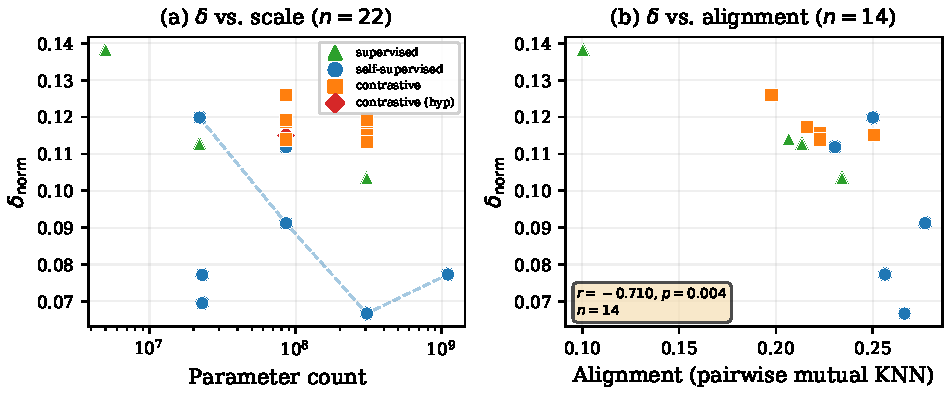
\includegraphics[width=\linewidth]{figures/fig1_alignment.pdf}
  \caption{(a)~$\delta$ vs.\ scale for 22 vision models: DINOv2 decreases with scale, supervised ViTs decrease moderately, contrastive models remain flat. (b)~$\delta$ vs.\ pairwise representation alignment ($n = 14$; $r = -0.710$, $p = 0.004$): more tree-like models align better with each other.}
  \label{fig:alignment}
\end{figure}

\paragraph{Cross-dataset generalization.} The $\delta$ ranking generalizes beyond ImageNet: correlations with ImageNet-Sketch ($r = 0.873$, $p < 10^{-6}$) and Places-365 ($r = 0.661$, $p < 0.001$) are highly significant. DINOv2 achieves the lowest $\delta$ on all three datasets. The weaker Places-365 correlation reflects its shallower taxonomy (365 scene categories vs.\ 1{,}000 object categories with deep WordNet hierarchy).

\subsection{Causal evidence: $\delta$ reflects learned hierarchy}
\label{sec:causal}

To distinguish architectural bias from learned structure, we run four interventions.

\paragraph{Random weights.} Random-initialized models have dramatically higher $\delta$: DINOv2-B ($+144\%$), DINOv2-S ($+134\%$), ViT-B ($+65\%$). The tree-like structure is not architectural.

\paragraph{Non-hierarchical fine-tuning.} Fine-tuning on a 8-class color classification task (no class hierarchy) increases $\delta$: CLIP-B ($+91\%$), DINOv2-S ($+69\%$), ViT-B ($+19\%$). Fine-tuning on hierarchical CIFAR-100 produces minimal change ($-8\%$ to $+6\%$). Same protocol, different task structure---only destroying hierarchy increases $\delta$.

\paragraph{Layer emergence.} $\delta$ decreases progressively from layer~1 to the final layer in pretrained transformers: DINOv2-B ($-60\%$), CLIP-B ($-46\%$). A randomly initialized ViT-B shows flat $\delta \approx 0.195$ throughout, ruling out architectural artifacts.

\paragraph{Shuffle control.} Shuffling preserves point-cloud geometry but destroys label-correspondence: $\delta$ does not change ($p > 0.12$). This confirms that $\delta$ measures \emph{semantic} organization, not a trivial property of high-dimensional point clouds.

\begin{figure}[t]
  \centering
  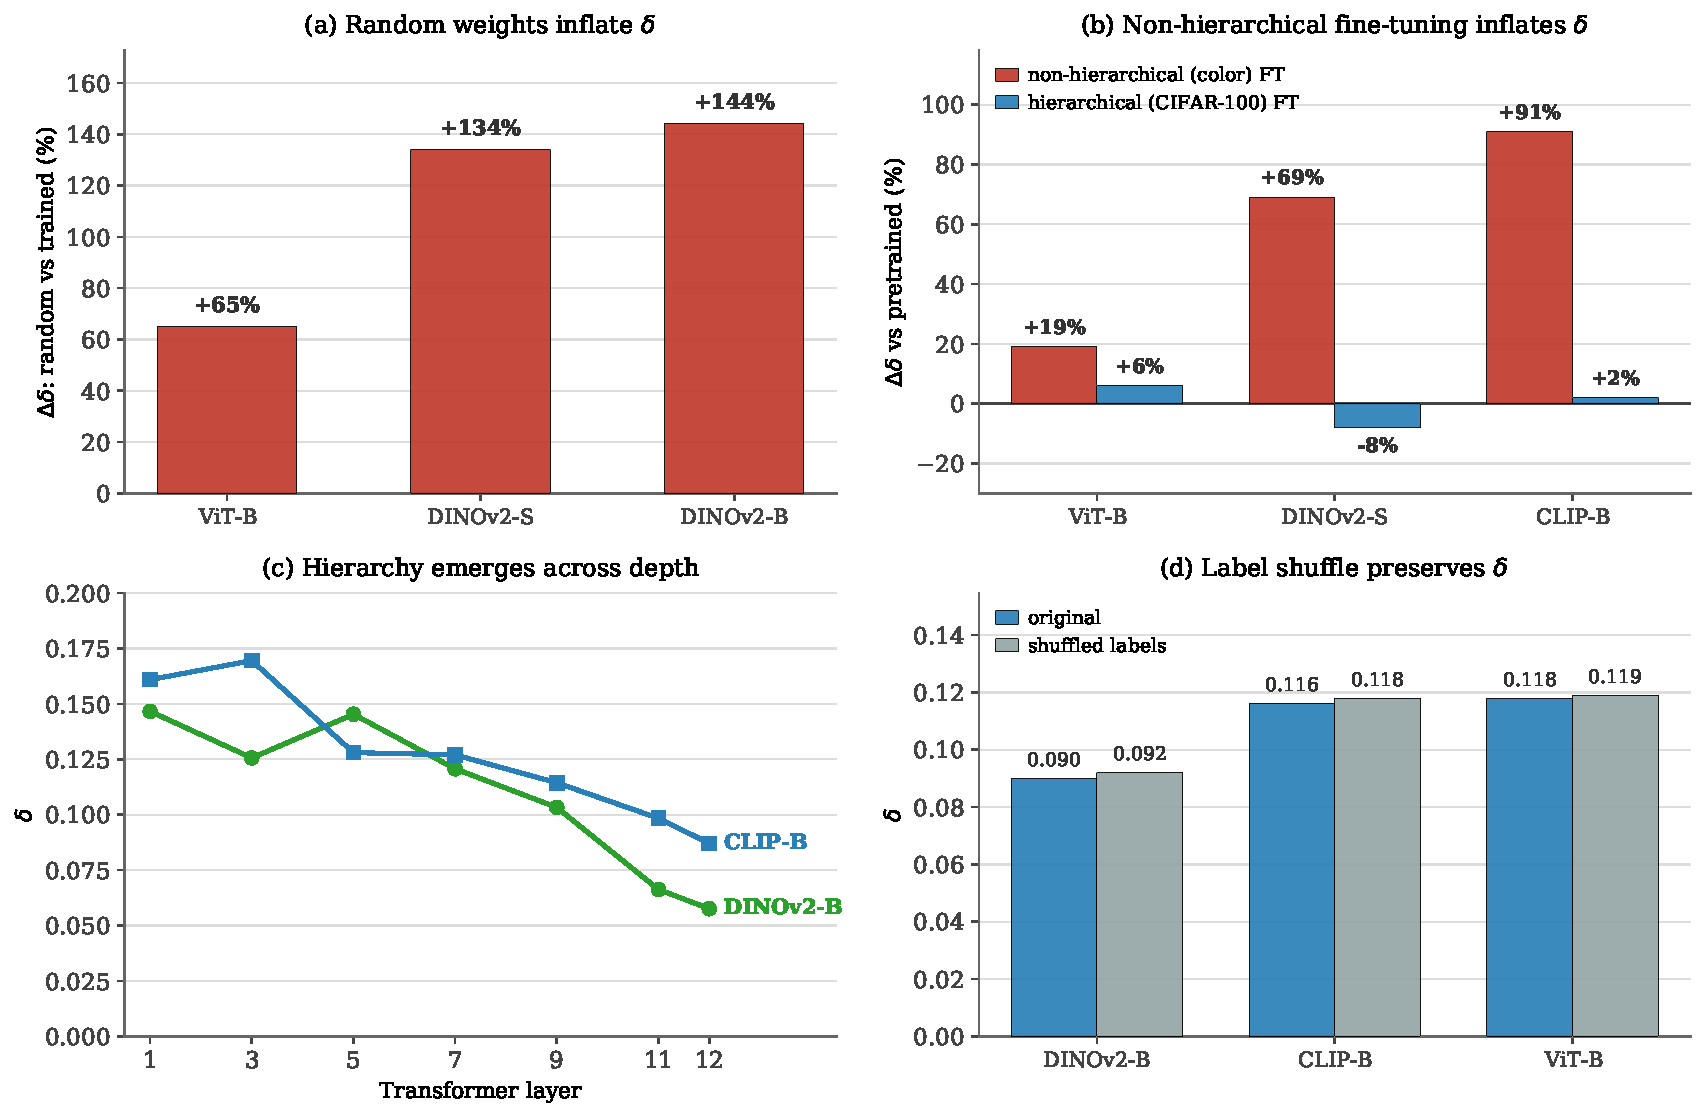
\includegraphics[width=\linewidth]{figures/fig3_causal.pdf}
  \caption{Causal evidence. (a)~Color fine-tuning (non-hierarchical) increases $\delta$ by 19--91\%. (b)~Shuffling embeddings preserves $\delta$ ($p > 0.12$). (c)~Random-weight models have 65--144\% higher $\delta$ than trained counterparts.}
  \label{fig:causal}
\end{figure}

\subsection{Geometric characterization}
\label{sec:geometry}

\paragraph{Three-way embedding distortion.} We embed 100 centroids per model into $\mathbb{R}^{10}$ (Adam-optimized stress) and $\mathbb{H}^{10}$ (Riemannian Adam), and compare against discrete-tree distortion (best of UPGMA, Ward, MST). Across all 40 models, $\mathbb{H}^{10}$ outperforms $\mathbb{R}^{10}$ ($\rho(\mathbb{H}/\mathbb{R}) > 1$ in 40/40 cases; range $1.03$--$1.21$). On ImageNet (deep WordNet taxonomy), discrete trees outperform $\mathbb{H}^{10}$ in 17/22 vision models---these representations are so tree-like that even continuous hyperbolic manifolds cannot fully capture them. On Places-365 (shallow taxonomy, 365 scene categories), $\mathbb{H}^{10}$ wins 18/22, indicating that the relative advantage of trees vs.\ continuous $\mathbb{H}^{10}$ depends on taxonomic depth.

\paragraph{Four-point defects.} Examining 100K random quadruples per model and comparing to synthetic references ($\mathbb{H}^{10}$, $\mathbb{R}^{10}$, $S^{10}$), three regimes emerge: (i)~\textbf{strongly hyperbolic} (DINOv2 family, GPT-2 XL, OLMo: defect 0.005--0.012, matching concentrated $\mathbb{H}^{10}$); (ii)~\textbf{moderately hyperbolic} (contrastive vision, text embeddings, supervised: defect 0.015--0.024); (iii)~all 40 models far from $\mathbb{R}^{10}$ ($0.037$) and $S^{10}$ ($0.057$).

\paragraph{Ollivier--Ricci curvature.} ORC~\citep{ollivier2009ricci} on the $k{=}10$ kNN graph correlates with $\delta$ across all 40 models ($r = -0.71$, $p < 10^{-4}$). DINOv2 has the highest ORC ($0.52$--$0.65$, 0\% negative edges), supervised models are moderate ($0.31$--$0.38$, 4--7\%), contrastive lower ($0.31$--$0.34$, 5--6\%). Causal LMs cluster with supervised (ORC $0.27$--$0.41$). Text embeddings show distinctly lower ORC ($0.17$--$0.24$), indicating uniformly hyperbolic geometry rather than sharp tree-like clustering. The ranking is preserved across $k \in \{5, 10, 15, 20, 30, 50\}$ (Spearman $r = 1.0$).

\subsection{Practical payoff: when post-hoc Poincar\'{e} projection helps}
\label{sec:practical}

The geometric characterization has a direct practical consequence: $\delta$ predicts when post-hoc projection of frozen-backbone features into the Poincar\'{e} ball improves prototype-based classification. We evaluate two parameter-free recipes on 12 vision models $\times$ 6 datasets---ImageNet (1{,}000 classes, 30 WordNet superclasses), CIFAR-100, CIFAR-10, DTD, FashionMNIST, MNIST---for a total of $n = 72$ combinations.

\paragraph{The pipeline.} For each (model, dataset): freeze the backbone; compute mean $\boldsymbol\mu$ and 95th-percentile norm $\rho_{95}$ on training features; choose scale $s = 2\,\mathrm{arctanh}(0.5)/\rho_{95}$; project every feature $\boldsymbol{x}$ via the exponential map at the origin, $\phi(\boldsymbol{x}) = \tanh(\|s(\boldsymbol{x}-\boldsymbol\mu)\|/2) \cdot s(\boldsymbol{x}-\boldsymbol\mu)/\|s(\boldsymbol{x}-\boldsymbol\mu)\|$. The scale ensures the 95th percentile of projected norms reaches $0.5$ in the unit Poincar\'{e} ball, avoiding shell collapse (where all features pile up against the boundary and Poincar\'{e} distance reduces to a function of angles only).

\paragraph{Task NC: Nearest-Centroid classification.} For each class $c$, compute the prototype as the mean of training features. Classify each test sample by argmin distance to prototypes. Pooling all 72 (model, dataset) combinations, the Pearson correlation between $\delta$ on the input centroids and the hyperbolic advantage $H_\text{adv} = (\mathrm{acc}_H - \mathrm{acc}_R) \times 100$ pp is $r = -0.542$ ($p < 10^{-6}$). Within each individual dataset the correlation is stronger (Table~\ref{tab:within-dataset}), reaching $r = -0.911$ on CIFAR-100 and $r = -0.740$ on ImageNet. DINOv2-L gains $+2.36$ pp on CIFAR-100, $+0.62$ pp on ImageNet.

\paragraph{Task FS: 5-way 5-shot few-shot.} 1{,}000 episodes per (model, dataset); per episode 5 classes, 5 support + 15 query each; classify queries by nearest support-prototype. Pooling all 72 combinations, Pearson $r = -0.496$ ($p < 10^{-5}$). \emph{Every} of the 12 models on ImageNet gains in few-shot ($H_\text{adv}$ from $+0.01$ to $+1.31$ pp), and the magnitude scales tightly with $\delta$: within ImageNet the correlation is $r = -0.868$ ($p = 0.0003$). DINOv2-L gains $+1.24$ on ImageNet, $+1.27$ on CIFAR-100, $+1.86$ on DTD.

\begin{figure}[t]
  \centering
  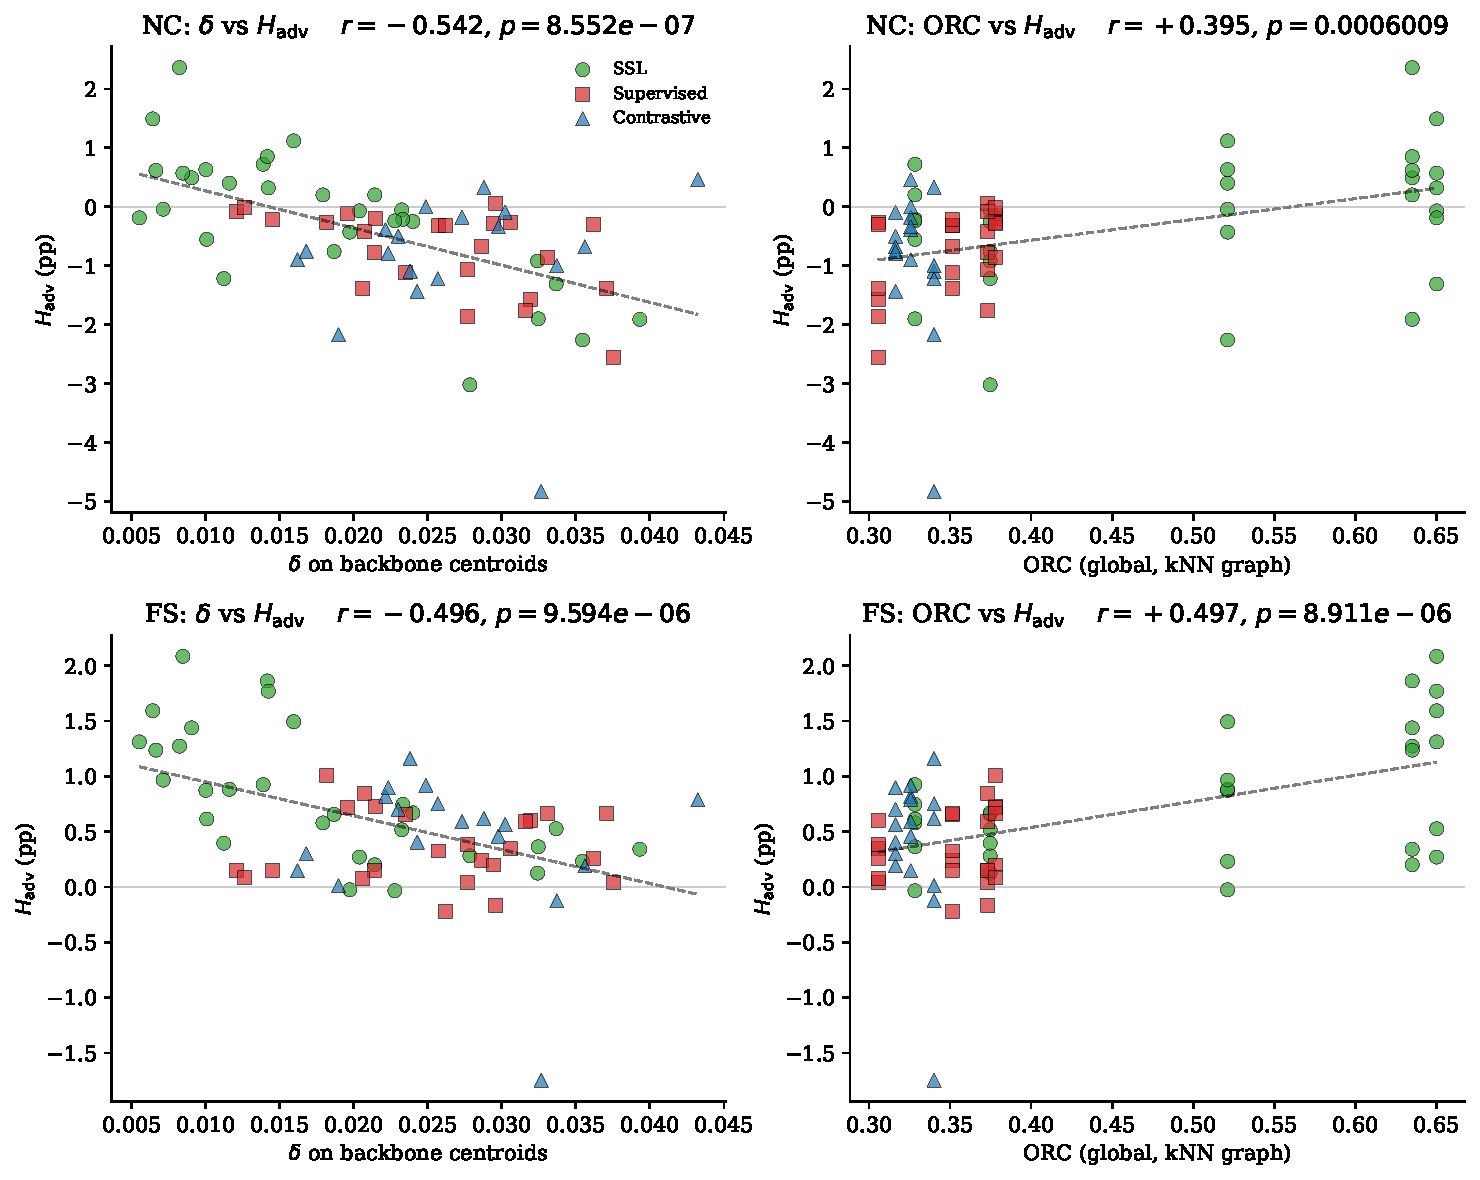
\includegraphics[width=\linewidth]{figures/fig_tasks_CE.pdf}
  \caption{$\delta$ predicts the hyperbolic advantage in post-hoc prototype-based downstream tasks (12 vision models $\times$ 5 datasets, $n = 60$). Left: nearest-centroid classification ($r = -0.629$). Right: 5-way 5-shot few-shot ($r = -0.604$, 1{,}000 episodes per combination). SSL backbones (lowest $\delta$) show the largest gains. Dashed line: linear fit.}
  \label{fig:tasks_CE}
\end{figure}

\paragraph{Within-dataset analysis.} The hyperbolic advantage requires hierarchical structure in \emph{both} the backbone (low $\delta$) and the labels. Within each dataset, Pearson correlations between $\delta$ and $H_\text{adv}$ across the 12 models (Table~\ref{tab:within-dataset}):

\begin{table}[h]
\centering\scriptsize
\caption{Within-dataset Pearson correlation $r$ between backbone $\delta$ and hyperbolic advantage $H_\text{adv}$, across 12 vision models. Datasets ordered by depth of label hierarchy.}
\label{tab:within-dataset}
\begin{tabular}{lccccl}
\toprule
Dataset & $r$ (NC) & $r$ (Few-shot) & $r$ (RetrFine) & $r$ (RetrSup) & Hierarchy \\
\midrule
ImageNet & $\mathbf{-0.740}^{**}$ & $\mathbf{-0.868}^{****}$ & $-0.062$ & $-0.038$ & 30 WordNet super \\
CIFAR-100 & $\mathbf{-0.911}^{****}$ & $\mathbf{-0.750}^{**}$ & $+0.244$ & $+0.290$ & 20 WordNet super \\
DTD & $\mathbf{-0.817}^{***}$ & $\mathbf{-0.919}^{****}$ & $+0.079$ & --- & emergent clusters \\
CIFAR-10 & $\mathbf{-0.622}^{*}$ & $\mathbf{-0.779}^{***}$ & $-0.047$ & $+0.129$ & vehicle / animal \\
FashionMNIST & $-0.567$ & $+0.112$ & $-0.209$ & $-0.299$ & weak (4 super) \\
MNIST & $+0.348$ & $+0.180$ & $-0.252$ & $-0.177$ & arbitrary \\
\bottomrule
\multicolumn{6}{l}{\scriptsize $^*p<0.05$, $^{**}p<0.01$, $^{***}p<0.005$, $^{****}p<0.001$.}
\end{tabular}
\end{table}

The four datasets with deep or emergent hierarchy (ImageNet, CIFAR-100, DTD, CIFAR-10) show strong, highly significant negative correlations for both NC and few-shot: low backbone $\delta \Rightarrow$ larger hyperbolic gain. Datasets with weak or arbitrary hierarchy (MNIST, FashionMNIST) show no significant correlation. Sample-to-sample retrieval shows no correlation in any dataset, confirming the asymmetry argument: H acts on the radial dimension of the ball, which is informative only when one side of the comparison is a clean prototype.

\paragraph{Negative result on symmetric retrieval.} For completeness we also evaluate sample-to-sample retrieval P@10 (12 models $\times$ 5 datasets) using the same projection. The hyperbolic advantage is uniformly negative or null across all paradigms (mean $-1.0$ to $-2.3$ pp), and the correlation with $\delta$ is reversed: $r = +0.30$ (fine class) and $r = +0.37$ (superclass), $n = 60$. Geometrically: when both query and database items are individual samples, no asymmetry exists between ``noisy'' and ``clean'' representations for the radial dimension of the Poincar\'{e} ball to encode. The hyperbolic advantage is therefore restricted to settings where one side is a clean class prototype (NC, few-shot)---a prediction that is borne out across paradigms and datasets.

\paragraph{Practical protocol.} Compute $\delta$ on training-set class centroids ($\sim$8 seconds CPU, 1{,}000 quadruples). \emph{If $\delta < 0.10$ and the labels carry a deep semantic hierarchy}, post-hoc Poincar\'{e} projection of frozen features improves NC and few-shot by $0.5$--$2.5$ pp; \emph{otherwise}, retain Euclidean. The decision is reversible (one-line distance switch), requires no training, and cannot be confounded by optimization or regularization tuning.

%% ============================================================
\section{Discussion}
\label{sec:discussion}
%% ============================================================

\paragraph{Implications for the PRH.} Our results add a geometric dimension to the Platonic Representation Hypothesis: models converge toward the same \emph{type} of space---one with tree-like inter-class distance structure. The reasoning is: reality has hierarchical structure $\rightarrow$ models learn that hierarchy $\rightarrow$ tree-like distances minimize distortion of that hierarchy $\rightarrow$ $\delta$ is low. Tree-like geometry is an independently interesting within-model property even if cross-model convergence is partially artifactual~\citep{groger2026revisiting}.

\paragraph{Universal tree-like geometry, two mechanisms.} All paradigms produce tree-like geometry, but via different mechanisms. Self-supervised vision models and causal LMs achieve the lowest $\delta$ with emergent hierarchies (low WN $r$). Contrastive models---vision and text alike---learn WordNet-aligned hierarchies with moderate $\delta$ (high WN $r$). The training objective, not the modality, determines the geometric signature.

\paragraph{When does H help?} Our practical results decompose the question. Hyperbolic projection helps iff (i)~the backbone's centroid distance structure is tree-like (low $\delta$), \emph{and} (ii)~the downstream task involves an asymmetric comparison between a noisy individual sample and a clean class representative (NC, few-shot), \emph{and} (iii)~the labels carry semantic hierarchy. In the absence of any one ingredient---e.g., symmetric sample-to-sample retrieval, or a label space without hierarchy like MNIST---H provides no advantage and may slightly hurt. This is consistent with the geometric mechanism: the radial dimension of the Poincar\'{e} ball encodes ``how typical / how peripheral'' a representation is, and that encoding is informative only when one side of the comparison is typical (a prototype) and the other can be peripheral (a sample).

\paragraph{Limitations.} Our $\delta$ analysis measures inter-class centroid geometry, not within-class or instance-level geometry. For self-supervised models, low $\delta$ is partly explained by the eigenvalue spectrum: a spectrum-matched null with the same eigenvalue distribution but randomized directions produces comparable $\delta$ for 7/22 vision models. The spectrum is itself learned (random weights produce different spectra and 65--144\% higher $\delta$), but the geometric interpretation is weaker than for contrastive models, where 15/22 show structural tree-likeness beyond spectral effects. Causal experiments use $n = 3$--$4$ models on CIFAR-100; extending strengthens the causal claims. The few-shot evaluation uses random class subsets within each dataset rather than a held-out novel-class split. Finally, no model satisfies the strict ultrametric inequality; representations are tree-\emph{like}, not perfect trees.

%% ============================================================
\section{Conclusion}
\label{sec:conclusion}
%% ============================================================

We have shown that hyperbolic geometry---measured as tree-like inter-class distance structure---is a universal property of learned representations. Across 39 models in five paradigms, $\mathbb{H}^{10}$ outperforms $\mathbb{R}^{10}$ in pairwise distance preservation in every case. Five geometric metrics ($\delta$, ORC, four-point defects, intrinsic dimension, three-way distortion) converge on the same characterization. Controlled experiments establish that this geometry reflects \emph{learned} semantic hierarchy: random weights, non-hierarchical fine-tuning, and layer-wise analysis all support a causal link between $\delta$ and hierarchy formation. The discovery that causal LMs are also tree-like overturns the assumption that this property is vision-specific.

Crucially, the geometry is not merely descriptive but \emph{prescriptive}. $\delta$ predicts when post-hoc Poincar\'{e} projection improves prototype-based classification ($r = -0.629$) and few-shot learning ($r = -0.604$), and when it does not (sample-to-sample retrieval, datasets without label hierarchy). Computing $\delta$ takes seconds on CPU, providing a zero-cost diagnostic that tells practitioners whether to use hyperbolic geometry on their specific backbone--dataset combination---and when not to.

\begin{ack}
[Acknowledgments hidden in anonymous submission.]
\end{ack}

%% ============================================================
\section*{References}

{\small
[1] Huh, M., Cheung, B., Wang, T., Isola, P. (2024) The Platonic Representation Hypothesis. \emph{ICML}.

[2] Gromov, M. (1987) Hyperbolic groups. In \emph{Essays in Group Theory}, MSRI Publ., 8:75-263.

[3] Nickel, M., Kiela, D. (2017) Poincar\'{e} embeddings for learning hierarchical representations. \emph{NeurIPS}.

[4] Sarkar, R. (2011) Low distortion delta-hyperbolic embedding of trees. In \emph{Graph Drawing}.

[5] Khrulkov, V., Mirvakhabova, L., Ustinova, E., Oseledets, I., Lempitsky, V. (2020) Hyperbolic image embeddings. \emph{CVPR}.

[6] Bdeir, A., Zou, B., Roussos, A., Davis, L., Mukhopadhyay, S. (2024) Fully hyperbolic convolutional neural networks. \emph{ICLR}.

[7] Desai, K., Nickel, M., Rajpurohit, T., Johnson, J., Vedantam, R. (2023) Hyperbolic image-text representations. \emph{ICML} (MERU).

[8] Ollivier, Y. (2009) Ricci curvature of Markov chains on metric spaces. \emph{J.\ Funct.\ Anal.} 256(3):810-864.

[9] Caron, M., Touvron, H., Misra, I., J\'{e}gou, H., Mairal, J., Bojanowski, P., Joulin, A. (2021) Emerging properties in self-supervised vision transformers. \emph{ICCV} (DINO).

[10] Oquab, M.\ et al.\ (2024) DINOv2: Learning robust visual features without supervision. \emph{TMLR}.

[11] Radford, A.\ et al.\ (2021) Learning transferable visual models from natural language supervision. \emph{ICML} (CLIP).

[12] Zhai, X., Mustafa, B., Kolesnikov, A., Beyer, L. (2023) Sigmoid loss for language-image pre-training. \emph{ICCV} (SigLIP).

[13] Dosovitskiy, A.\ et al.\ (2021) An image is worth 16$\times$16 words. \emph{ICLR} (ViT).

[14] Biderman, S.\ et al.\ (2023) Pythia: A suite for analyzing large language models. \emph{ICML}.

[15] Groger, F.\ et al.\ (2026) Revisiting the Platonic Representation Hypothesis. (concurrent).
}

%% ============================================================
\appendix
\section{Additional model details and ablations}
Full results for all 39 models across $\delta$, ORC, defects, three-way distortion, and within-dataset task analyses are provided in the supplementary CSVs. We also include rank-matched and spectrum-matched null analyses (15/22 vision models pass spectrum-matched null at $p < 0.05$).

\newpage
\input{checklist.tex}

\end{document}
